%-*-latex-*-
\sectionthree{Example: height computation}
\begin{python0}
from solutions import *; clear()
\end{python0}

Let me do a simple example.
Let's talk about the height.
Look at this:
\begin{center}
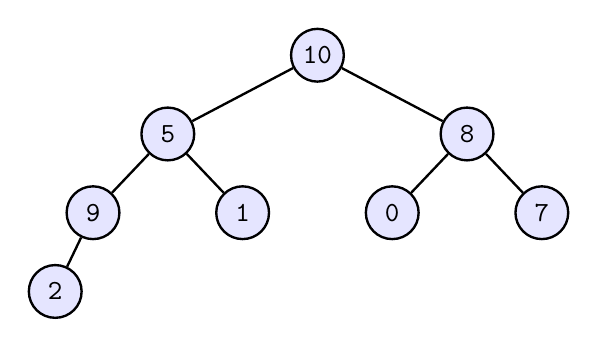
\begin{tikzpicture}

\fill[blue!10] (0.0, 0.0) circle (0.35);
\node [line width=0.03cm,black,minimum size=0.6699999999999999cm,draw,circle] at (0.0,0.0)(10){};\draw (0.0, 0.0) node[color=black] {\texttt{10}};
\fill[blue!10] (-1.9, -1.0) circle (0.35);
\node [line width=0.03cm,black,minimum size=0.6699999999999999cm,draw,circle] at (-1.9,-1.0)(5){};\draw (-1.9, -1.0) node[color=black] {\texttt{5}};
\fill[blue!10] (1.9, -1.0) circle (0.35);
\node [line width=0.03cm,black,minimum size=0.6699999999999999cm,draw,circle] at (1.9,-1.0)(8){};\draw (1.9, -1.0) node[color=black] {\texttt{8}};
\fill[blue!10] (-2.85, -2.0) circle (0.35);
\node [line width=0.03cm,black,minimum size=0.6699999999999999cm,draw,circle] at (-2.85,-2.0)(9){};\draw (-2.85, -2.0) node[color=black] {\texttt{9}};
\fill[blue!10] (-0.95, -2.0) circle (0.35);
\node [line width=0.03cm,black,minimum size=0.6699999999999999cm,draw,circle] at (-0.95,-2.0)(1){};\draw (-0.95, -2.0) node[color=black] {\texttt{1}};
\fill[blue!10] (0.95, -2.0) circle (0.35);
\node [line width=0.03cm,black,minimum size=0.6699999999999999cm,draw,circle] at (0.95,-2.0)(0){};\draw (0.95, -2.0) node[color=black] {\texttt{0}};
\fill[blue!10] (2.85, -2.0) circle (0.35);
\node [line width=0.03cm,black,minimum size=0.6699999999999999cm,draw,circle] at (2.85,-2.0)(7){};\draw (2.85, -2.0) node[color=black] {\texttt{7}};
\fill[blue!10] (-3.33, -3.0) circle (0.35);
\node [line width=0.03cm,black,minimum size=0.6699999999999999cm,draw,circle] at (-3.33,-3.0)(2){};\draw (-3.33, -3.0) node[color=black] {\texttt{2}};\draw[line width=0.03cm,black] (10) to  (5);
\draw[line width=0.03cm,black] (10) to  (8);
\draw[line width=0.03cm,black] (5) to  (9);
\draw[line width=0.03cm,black] (5) to  (1);
\draw[line width=0.03cm,black] (8) to  (0);
\draw[line width=0.03cm,black] (8) to  (7);
\draw[line width=0.03cm,black] (9) to  (2);
\end{tikzpicture}

\end{center}



The height of the tree (or the height of $a$) is 3.
The \defone{height} of $a$ is defined to the length of the 
longest path from $a$ to the leaves.

Let's think about the height recursively.
We break up the tree (at $a$) into the left subtree $L$ (subtree at $b$),
the root $a$, and the right subtree $R$ (subtree at $d$).
A longest path from $a$ must either go into $L$ or into $R$.
Let's look at $L$ first.

Of course there's an edge from $a$ into $L$.
If the longest path from $a$ to a leaf actually went into $L$,
then the longest path, after removing the edge from $a$ to $b$,
would also be a longest path for $b$ to a leaf.
Clearly if this is the case,
\[
\operatorname{height}(a) = 1 + \operatorname{height}(b)
\]

Of course it could be the case that the longest path from $a$
actually went into $R$.
In that case, we have the similar fact:
\[
\operatorname{height}(a) = 1 + \operatorname{height}(d)
\]
By definition $\operatorname{height}(a)$ is the larger of the two.
So we get:
\[
\operatorname{height}(a) = 1 + \max(
\operatorname{height}(b),
\operatorname{height}(d))
\]
It should be clear now that if $n$ is any node,
\[
\operatorname{height}(n) = 1 + \max(
\operatorname{height}(n.\operatorname{left}),
\operatorname{height}(n.\operatorname{right}))
\]
So the function to compute height is probably something like this:
\begin{console}
ALGORITHM: height
INPUT:     node

if ???:
    return ???
else:
    return 1 + max(height(node.left), height(node.right))
\end{console}

Now for the base case.
If you want a single-node tree to be the base (look at node $k$ above),
then clearly the height of such a tree is 0.
\begin{console}
ALGORITHM: height
INPUT:     node

if node.is_leaf(): ??? DOES THIS WORK ???
    return 0
else:
    return 1 + max(height(node.left), height(node.right))
\end{console}
But you'll see that you get into some nasty ugliness.
To be concrete, think of the case of using C++ so that 
the above function accept \verb!p!, a pointer to node.
The problem is when \verb!p->left! might be \verb!NULL! -- 
and our base case does not include this case!!!
We stopped earlier, before we reach a \verb!NULL! pointer.
This means that I have to do this:
\begin{console}
ALGORITHM: height
INPUT:     node

if node.is_leaf():
    return 0
else:
    if node does not have a left child:
        return 1 + height(node.right))
    else if node does not have a right child:
        return 1 + height(node.left))
    else: 
        return 1 + max(height(node.left), 
                       height(node.right))
\end{console}
Nothing wrong with that!!! ... 
but let me show you a cleaner way.

If we include the \verb!NULL! pointer as a tree
then we'll need to define the height of an empty tree.
Our intuition tells us that
\verb!height(NULL)! should be $-1$.
But the important thing is the recursion:
\[
\operatorname{height}(\operatorname{node}) = 1 + \max(
\operatorname{height}(\operatorname{node.left}),
\operatorname{height}(\operatorname{node.right}))
\]
In other words, \verb!height(NULL)! is whatever we want it to be
as long as it satisfies the recursion.
If we set \verb!height(NULL) = -1! then 
this makes sense because for instance if you look at node $k$
which should have height 0, if you look at this:
\[
\operatorname{height}(k) = 1 + \max(
\operatorname{height}(\operatorname{NULL}),
\operatorname{height}(\operatorname{NULL}))
\]
you do get
\[
\operatorname{height}(k) = 1 + \max(-1, -1) = 0
\]
You can also verify for yourself that if a node has a left child
but no right child, then the above recursion also makes sense.

With this base condition, we have the following when
I'm using \verb!NONE! as a sort of fake sentinel node
that is attached to a node at the left is it does not have a left child
and to the right if the node does not have a right child.
\begin{console}
ALGORITHM: height
INPUT:     node

if node is NONE:
    return -1
else:
    return 1 + max(height(node.left), height(node.right))
\end{console}
The subtree with a node of \verb!NONE! is just the empty tree.

Obviously the C++ code is this:
{\small
\begin{console}
int height(const Node * const p)
{
    if (p == NULL)
    {
        return -1;
    }
    else
    {
        return 1 + max(height(p->left), height(p->right));
    }
}
\end{console}
}
(Why the two \verb!const!? 
The pointer value does not have and the attributes of the node
does not change.)

What you should take away from the above
is this: 
in terms of 
recursive--thinking, for tree computations it's cleaner
to include the case of an empty tree.
In other words we \textit{do} want an empty graph to be a tree too.
The definition of a tree should therefore be the following:
$T$ is a tree if
\begin{itemize}
\li $T$ is an empty tree, or
\li $T$ has a root node with children $T_1, ..., T_k$ 
where each $T_i$ is a tree.
\end{itemize}
In the case of binary tree this means that a recursion
function \verb$F$ might have this shape:
\begin{console}
ALGORITHM: F
INPUT:     node

if node is NONE:
    ...
else:
    DO SOMETHING WITH node, F(node.left), F(node.right)
\end{console}

\begin{ex}
Analyze the \verb!size()! method and write down the
pseudocode. Implement it in C++.
\qed
\end{ex}

\begin{ex}
Analyze the \verb!depth()! function and write down the
pseudocode. Of course you have to assume that 
each node has a parent pointer.
Implement it in C++.
\qed
\end{ex}

